\section{Лекция от 21.04.2018}
\begin{theorem}[о монотонной сходимости][б/д]
	Пусть $\{\xi_n\}_{n \geqslant 1}, \xi, \eta$~--- случайные величины, тогда
	\begin{enumerate}
		\item {Если $\xi_n \uparrow \xi$ почти наверное и $ \forall n \in \N: \xi_n \geqslant \eta, \E \eta > - \infty$, то $\E \xi = \lim\limits_{n \rightarrow \infty} \E \xi_n$.}
		\item {Eсли Если $\xi_n \downarrow \xi$ почти наверное и $ \forall n \in \N: \xi_n \leqslant \eta, \E \eta < + \infty$, то $\E \xi = \lim\limits_{n \rightarrow \infty} \E \xi_n$.}
	\end{enumerate}
\end{theorem}
\begin{lemma}[Фату]
	Пусть $\{ \xi_n \}_{n \geqslant 1}$ и $\eta$~--- случайные величины, $\E | \eta| < + \infty$, тогда 
	\begin{enumerate}
		\item { Если $\forall n: \xi_n \geqslant \eta$, то $ \varliminf\limits_{n \rightarrow \infty} \E \xi_n \geqslant \E \varliminf\limits_{n \rightarrow \infty} \xi_n$.}
		\item { Если $\forall n: \xi_n \leqslant \eta$, то $ \varlimsup\limits_{n \rightarrow \infty} \E \xi_n \leqslant \E \varlimsup\limits_{n \rightarrow \infty} \xi_n$.}
		\item { Если $\forall n: |\xi_n| < \eta$, то $ \E \varliminf\limits_{n \rightarrow \infty} \xi_n \leqslant \varliminf\limits_{n \rightarrow \infty} \E \xi_n \leqslant \varlimsup\limits_{n \rightarrow \infty} \E \xi_n \leqslant \E \varlimsup\limits_{n \rightarrow \infty} \xi_n$.}
	\end{enumerate}
	\begin{proof}
		(1) Обозначим $\psi_n = \inf\limits_{k \geqslant n} \xi_k$. Очевидно, $\psi_n \uparrow \varliminf\limits_{n \rightarrow \infty} \xi_n$. кроме того $\psi_n \geqslant \eta$, следовательно, по теореме о монотонносй сходимости $ \lim\limits_{n \rightarrow \infty} \E \psi_n = \E \varliminf\limits_{n \rightarrow \infty} \xi_n$. Рассмотрим 
		$$\E \varliminf\limits_{n \rightarrow \infty} \xi_n = \lim\limits_{n \rightarrow \infty} \E \psi_n = \varliminf\limits_{n \rightarrow \infty} \E \psi_n \overset{\text{т.к.}~\psi_n \leqslant \xi_n}{\leqslant} \varliminf\limits_{n \rightarrow \infty} \E \xi_n.$$
		
		(2) Следует из пункта (1) заменой $\xi'_n = - \xi_n$.
		
		(3) Следует из (1) и (2).
	\end{proof}
\end{lemma}
\begin{theorem}[Лебега о мажорируемой сходимости]
	Пусть $\xi_n \xrightarrow{\text{п.н.}} \xi, |\xi| \leqslant \eta, \E \eta < + \infty$. Тогда $\E \xi_n \limn \E\xi$ и $\E | \xi_n - \xi| \limn 0$.
	\begin{proof}
		Заметим, что $\xi \overset{\text{п.н.}}{=} \lim\limits_{n \rightarrow \infty} \xi_n = \varliminf\limits_{n \rightarrow \infty} \xi_n = \varlimsup\limits_{n \rightarrow \infty} \xi_n$. По пункту (3) леммы Фату
		\begin{multline*}
			\E \xi = \E \varliminf\limits_{n \rightarrow \infty} \xi_n \leqslant \varliminf\limits_{n \rightarrow \infty} \E \xi_n \leqslant \varlimsup\limits_{n \rightarrow \infty} \E \xi_n \leqslant  \E \varlimsup\limits_{n \rightarrow \infty} \xi_n  = \E \xi \quad \Rightarrow \quad \E \xi = \lim\limits_{n \rightarrow \infty} \xi_n.
		\end{multline*}
		Конечность $\E \xi$ следует из того, что $|\xi| < \eta$ почти наверное, следовательно, так как $\E \eta < + \infty$, то $\E |\xi| \leqslant \E | \xi | < + \infty$.
		
		Докажем $L_1$-сходимость. Возьмем $\psi_n = |\xi_n - \xi|$. Тогда $|\psi_n| \leqslant 2 \eta$ почти наверное и $\psi_n \xrightarrow{\text{п.н.}} 0$, следовательно, $\E \psi_n \limn 0$ по теореме Лебега.
	\end{proof}
\end{theorem}
\subsection{Сходимость в $L_2$}
Введем пространство $L_2 = L_2(\Omega, \F, \P) = \{ \xi: \E \xi^2 < + \infty \}$. Это минимальное пространство, так как $\E ( a \xi + b \eta)^2 \leqslant 2 a^2 \E\xi^2 + 2b^2\E\eta^2$. \\

Основное неравенство: $(x+y)^2 \leqslant 2x^2 + 2y^2$.\\

Норма $ \| \xi \| = \sqrt{\E \xi^2}$;  скалярное произведение $(\xi, \eta) = \E \xi\eta$.
\begin{lemma}
	Пусть $\xi_n \xrightarrow{L_2} \xi$, $\forall n: \xi_n \in L_2$. Тогда
	\begin{enumerate}
		\item $\xi \in L_2$,
		\item $E\xi_n \limn \E \xi$,
		\item $\E \xi_n^2 \limn \E\xi^2$,
		\item {если $\eta_n \xrightarrow{L_2} \eta$, $\forall n: \eta_n \in \L_2$, то $(\xi_n, \eta_n) \limn (\xi, \eta)$.}
	\end{enumerate}
	\begin{proof}
		Докажем первый пункт леммы:
		$$\E \xi^2 = \E ( \xi - \xi_n + \xi_n)^2 \leqslant \underbracket[0.5pt]{2\E( \xi - \xi_n)^2}_{\rightarrow 0} + \underbracket[0.5pt]{2\E \xi_n^2}_{< + \infty} < +\infty.$$
		Перейдем ко второму пункту. Если $\E \xi^2 < + \infty$, то $\E | \xi | = \E | \xi| \cdot 1$, а по неравенству Коши-Буняковского это меньше или равно, чем $\sqrt{\E \xi^2 \cdot \cancelto{1}{\E 1^2}} < + \infty$. Осталось заметить, что $\big| \E ( \xi_n - \xi ) \big| \leqslant \E | \xi_n - \xi | \leqslant \sqrt{\E (\xi_n - \xi)^2 \cdot E 1^2} \limn 0$.
		Пункт 3. 
		\begin{multline*}
			\E ( \xi_n^2 - \xi^2) = 
			\E ( \xi_n + \xi)(\xi_n - \xi) \leqslant \sqrt{ \E (\xi_n + \xi)^2 (\xi_n - \xi)^2} \leqslant \\ \leqslant
			 \sqrt{\big( \underbracket[0.5pt]{2 \E( \xi_n - \xi)^2}_{\rightarrow 0} + \underbracket[0.5pt]{8\E \xi^2}_{=\const} \cdot \underbracket[0.5pt]{\E (\xi_n^2 - \xi^2)}_{\rightarrow 0}} \limn 0.
		\end{multline*}
		Остается доказать четвертый пункт леммы:
		\begin{multline*}
			\E ( \xi_n \eta - \xi \eta) = 
			\E( \xi_n \eta_n - \xi_n \eta) + \E( \xi_n \eta - \xi \eta) \leqslant  \\ \leqslant
			\sqrt{\E\xi^2 \cdot \underbracket[0.5pt]{\E (\eta_n - \eta)^2}_{\rightarrow 0}} + \sqrt{\E \eta^2 \cdot \underbracket[0.5pt]{\E(\xi_n - \xi)^2}_{\rightarrow 0}} \limn 0.
		\end{multline*}
	\end{proof}
\end{lemma}
\subsection{Случайные блуждания и закон повторного логарифма}
Пусть $\{ \xi_i\}_{i \geqslant 1}$~--- последовательность независимых одинаково распределенных случайных величин таких, что $\E \xi_n = 0, \E \xi_n^2 = \sigma^2$.
\begin{definition}
	Случайная величина $S_n = \sum\limits_{i = 1}^n \xi_i$ называется случайным блужданием.
\end{definition}
Известно (из Ц.П.Т.), что $ \varlimsup\limits_{n \rightarrow \infty} \dfrac{S_n}{\sqrt{n}} = + \infty$, а $ \varliminf\limits_{n \rightarrow \infty} \dfrac{S_n}{\sqrt{n}} = - \infty$. С другой стороны,
$$ \sum\limits_{n = 1}^\infty \dfrac{\E \xi_n^2}{n \ln^2 n} = \sum\limits_{n = 1}^\infty  \frac{\sigma^2}{n \ln^2 n} < + \infty.$$
Следовательно, по теореме Колмогорова-Хинчина о сходимости ряда почти наверное $\sum\limits_{n = 1}^\infty \dfrac{\xi_n}{\sqrt{n} \ln^2 n}$ сходится почти наверное, значит, по лемме Кронекера, 
$$ \dfrac{1}{\sqrt{n} \ln n} \sum\limits_{k = 1}^n \sqrt{k} \ln k \dfrac{\xi_k}{ \sqrt{k} \ln k} = \dfrac{S_n}{\sqrt{n} \ln n} \xrightarrow[n \rightarrow \infty]{\text{п.н.}} 0.$$
\begin{definition}
	Функция $\varphi^* = \varphi^*(n)$, $n > 1$ называется верхней для $S_n$, если $S_n(\omega) < \varphi^*(n)$ почти наверное для всех $n$, начиная с некоторого $n_0(\omega)$.
\end{definition}
\begin{definition}
	Функция $\varphi_* = \varphi_*(n)$, $n > 1$ называется нижней для $S_n$, если $S_n(\omega) > \varphi_*(n)$ почти наверное для бесконечно многих $n$ (бесконечно часто).
\end{definition}
То есть $\varphi^* (n) = \varepsilon \sqrt{n} \ln n$~--- верхняя для произвольного случайного блуждания, $\varphi_* (n) = \varepsilon \sqrt{n}$~--- нижняя. Пусть $\varphi(n)$~--- <<точная асимптотика>>, возьмем $\varphi_\varepsilon^* = (1 + \varepsilon) \varphi^*; \varphi_{*\varepsilon} = (1 - \varepsilon) \varphi$ для $\varepsilon > 0$. Тогда 
	\begin{multline*}
		\left\{ \varlimsup\limits_{n \rightarrow \infty} \dfrac{S_n}{\varphi(n)} \leqslant 1 \right\} = 
		\left\{ \lim\limits_{n \rightarrow \infty} \sup\limits_{m \geqslant n} \dfrac{S_m}{\varphi(m)} \leqslant 1 \right\} = \\ =
		\left\{ \forall \varepsilon > 0~\text{и некоторого}~n_\varepsilon: \sup\limits_{m \geqslant n_\varepsilon} \dfrac{S_n}{\varphi(m)} \leqslant 1 + \varepsilon \right\} = \\ =
		\big\{ \forall \varepsilon > 0~~\forall m \geqslant n_\varepsilon: S_m \leqslant (1 + \varepsilon) \varphi(m) \big\} \quad \Leftrightarrow \quad 
		(1 + \varepsilon) \varphi(m)~\text{--- верхняя.}
	\end{multline*}
Аналогично,
	\begin{multline*}
		\left\{ \varlimsup\limits_{n \rightarrow \infty} \dfrac{S_n}{\varphi(n)} \geqslant 1 \right\} = 
		\left\{ \lim\limits_{n \rightarrow \infty} \sup\limits_{m \geqslant n} \dfrac{S_m}{\varphi(m)} \geqslant 1 \right\} = \\ =
		\big\{ \forall \varepsilon > 0~\text{и для беск. многих}~n_\varepsilon: S_m \geqslant (1 - \varepsilon) \varphi(m) \big\}  \Leftrightarrow \\ \Leftrightarrow (1 - \varepsilon) \varphi(m)~\text{--- нижняя.}
	\end{multline*}

Отметим, $\forall \varepsilon > 0: \varphi_\varepsilon^* = (1 + \varepsilon) \varphi~\text{--- верхняя} \quad \Leftrightarrow \quad  \P\left( \varlimsup\limits_{n \rightarrow \infty} \dfrac{S_n}{\varphi(n)} \leqslant 1 \right) = 1$. Аналогично, $\forall \varepsilon > 0: \varphi_\varepsilon^* = (1 + \varepsilon) \varphi~\text{--- нижняя} \quad \Leftrightarrow \quad  \P\left( \varliminf\limits_{n \rightarrow \infty} \dfrac{S_n}{\varphi(n)} \geqslant 1 \right) = 1$.
\begin{theorem}[закон повторного логарифма (ЗПЛ)][б/д]
	Пусть $\{ \xi_n \}_{n \geqslant 1}$~--- независимые одинаково распределенные случайные величины, $\E \xi_1 = 0, \E \xi_1^2 = \sigma^2, 0 < \sigma^2 < + \infty$. Тогда 
	$$ \P \left( \varlimsup\limits_{n \rightarrow \infty} \dfrac{S_n}{\varphi(n)} = 1 \right) = 1,  \varphi(n) = \sqrt{
	2 \sigma^2 n \ln\ln n}. $$
\end{theorem}
\begin{note}
	Применяя ЗПЛ к $S_n$, получаем, что $\P \left(\varliminf\limits_{n \rightarrow \infty} \dfrac{S_n}{\varphi(n)} = -1 \right) = 1$.
\end{note}

За нижнюю ветку $S_n$ выходит бесконечно часто (см.~Рис.\,\ref{pic:lrl}), а за верхнюю лишь конечное число раз (почти наверное не выходит).
\begin{figure}[h!]
	\centering
	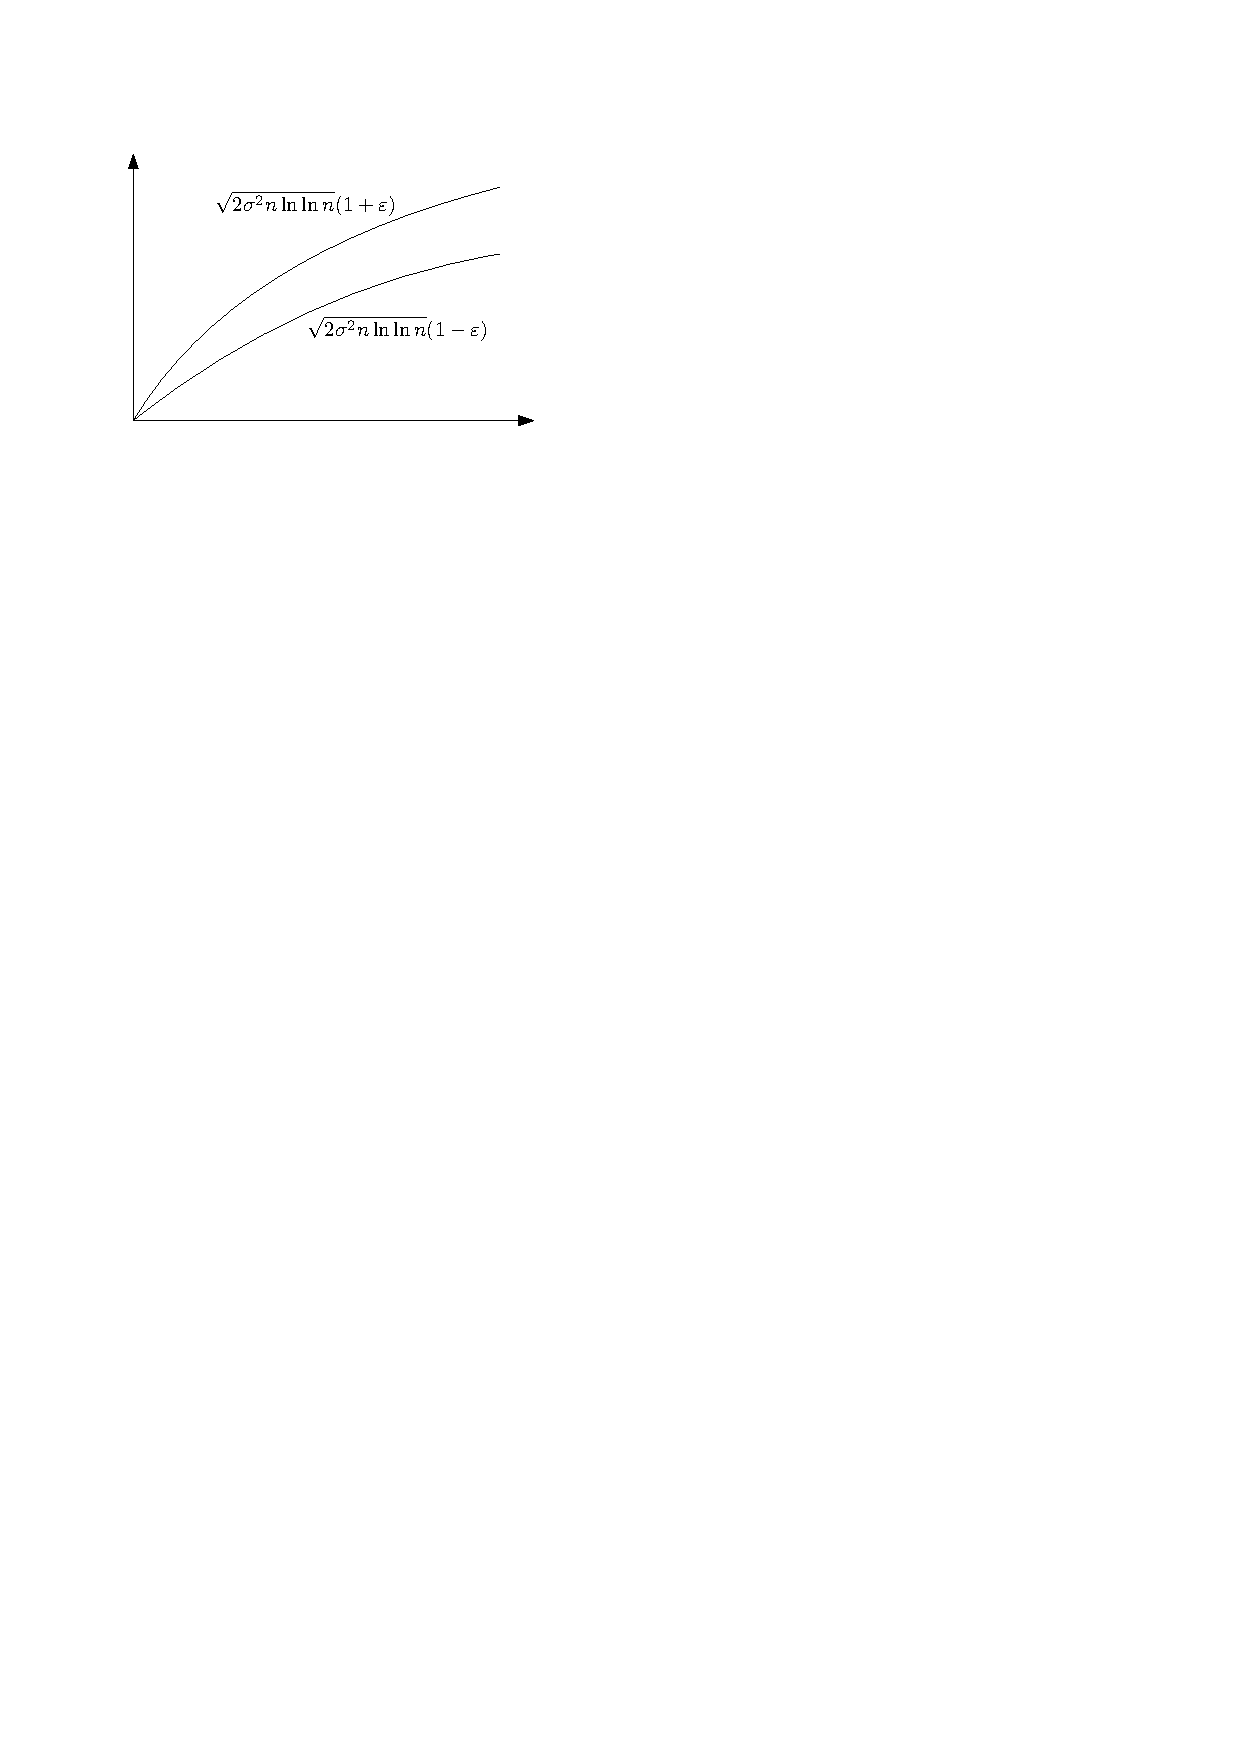
\includegraphics[width = 7cm]{lrl}
	\caption{Поведение верхней и нижней функции случайного блуждания}
	\label{pic:lrl}
\end{figure}
\subsection{Характеристические функции}
\begin{definition}
	Характеристическое функцией случайной величины $\xi$ называется $\varphi_\xi(t) = \E e^{it\xi}, t \in \R$.
\end{definition}
\begin{definition}
	Пусть $F(x)$~--- функция распределения, тогда ее характеристическая функция $\varphi_F (t) = \int\limits_\R e^{i t x} \, d F(x)$.
\end{definition}
 Если $F_\xi(x)$~--- функция распределения случайной величины $\xi$, то характеристические функции $\xi$ и $F_\xi$ совпадают.\\
 
 По формуле Эйлера $\varphi_\xi(t) = \E e^{i t \xi} = \E \cos (t \xi) + i \E \sin(t \xi)$.
 
 \begin{definition}
 	Пусть $\vec \xi = ( \xi_1, \ldots, \xi_n)$~--- случайный вектор. Его характеристической функцией называется $\varphi_{\vec \xi} \left(\vec t \right) = \E e^{i \left( \vec t, \vec \xi \right)}, t \in \R^n$.
 \end{definition}
 \begin{definition}
 	Пусть $F \left( \vec x \right), \vec x \in \R^n$~--- функция распределения в $\R^n$, тогда его характеристической функцией называется $\varphi_F \left( \vec t \right) = \int\limits_\R e^{i \left( \vec t, \vec x \right)} \, d F \left( \vec x \right), \vec x \in \R^n$.
 \end{definition}
 \subsection{Свойства характеристических функций}
 \setcounter{property}{0}
 \begin{property}
 	Пусть $\varphi(t)$~--- характеристическая функция случайной величины $\xi$, тогда $| \varphi (t) | \leqslant \varphi(0) = 1$.
 	\begin{proof}
 		$| \varphi(t) | = | \E e^{i t \xi} | \leqslant \E | \underbracket[0.5pt]{e^{i t \xi}}_{\equiv 1} | = 1 = \varphi(0)$.
 	\end{proof}
 \end{property}
	 






































